\documentclass{simcenterdocumentation}


\usepackage[backend=biber]{biblatex}
%\usepackage{subfig}
\usepackage{subcaption}
\usepackage{multirow}
\usepackage{adjustbox}
\usepackage{cleveref}
\usepackage{longtable}
\usepackage{draftwatermark}

\usepackage{hhline}
\usepackage{color, colortbl}
\definecolor{lightgray}{HTML}{E5E4E2}

\graphicspath{{../Common/}{.}} %Setting the graphicspath
\makeatletter % Search additional directories for inputs
\def\input@path{{../Common/}{.}}
%or: \def\input@path{{/path/to/folder/}{/path/to/other/folder/}}
\makeatother

%% Add unicode support for special characters
%%\usepackage[utf8x]{inputenc}

% To compile this file, run "latex/pdflatex codedoc", then "biber codedoc"b
% (or "bibtex codedoc", if the output from latex asks for that instead),
% and then "latex/pdflatex codedoc" (without the quotes in each case).

% Double spacing, if you want it.  Do not use for the final copy. Can also specify
% draft as a document class option. This will generate double spacing and placeholders
% for title page and header images
%% \def\dsp{\def\baselinestretch{2.0}\large\normalsize}
%% \dsp

\bibliography{../Common/references}

\begin{document}
% Declarations for Front Matter
% Software title followed by optional second line
\title{SimCenter Software Architecture}
% Use superscripts to indicate author affiliations
\author{Frank McKenna}
\institutions{NHERI SimCenter, UC Berkeley}
\softwarename{SA}
\softwareversion{1.0}

%%% DON'T MESS WITH THESE SETTINGS %%%%%%%%%%%%%%%%%%%%%%%%%%%%%%%%
\hypersetup{pageanchor=false}
\maketitle
\acknowledgments

\hypersetup{pageanchor=true}
\begin{frontmatter}

\pagestyle{plain}
{
  \renewcommand{\thispagestyle}[1]{}
  \tableofcontents
  \clearpage
  \listoffigures
  \clearpage
  \listoftables
}

\end{frontmatter}
\pagestyle{somewhatsimple}
%%%%%%%%%%%%%%%%%%%%%%%%%%%%%%%%%%%%%%%%%%%%%%%%%%%%%%%%%%%%%%%%%%%
% Create separate tex files for each chapter and provide them as inputs

\chapter{About}
\label{chap:about}
The audience of this tool is researchers and practitioners trying to
predict the response of a structure to earthquakes.\\

This open-source research application
(\href{https://github.com/NHERI-SimCenter/EE-UQ}{https://github.com/NHERI-SimCenter/EE-UQ})
provides an application researchers can use to predict the response of
a building subjected to earthquake events. The application is focused
on quantifying the uncertainties in the predicted response, given the
that the properties of the buildings and the earthquake events are not
known exactly, and that the simulation software and the user make
simplifying assumptions in the numerical modeling of that
structure. In the application, the user is required to characterize
the uncertainties in the input. The application will after utilizing
the selected sampling method, will provide information that
characterizes the uncertainties in the response measures. The
computations to make these determinations can be prohibitively
expensive. To overcome this impediment the user has the option to
perform the computations on the Stampede2 supercomputer. Stampede2 is
located at the Texas Advanced Computing Center and made available to
the user through NHERI DesignSafe, the cyberinfrastructure provider
for the distributed NSF funded Natural Hazards in Engineering Research
Infrastructure (NHERI) facility.\\

The computations are performed in a workflow application. That is, the
numerical simulations are actually performed by a number of different
applications. The EE-UQ backend software runs these different
applications for the user, taking the outputs from some programs and
providing them as inputs to others. The design of the EE-UQ
application is such that researchers are able to modify the backend
application to utilize their own application in the workflow
computations. This will ensure researchers are not limited to using
the default applications we provide and will be enthused to provide
their own applications for others to use. \\

This is Version 2.0 of the tool. Researchers are encouraged to comment on what additional
features and applications they would like to see in this
application. If you want it, chances are many of your colleagues also
would benefit from it.\\
\\


\chapter{Research Applications}
\label{chap:about}


The SimCenter is developing a software framework for building scientific workflow applications to perform computational; simulations in field of NHE at both building level scale and regionsl scale. It is releasing a number of applications built using this framework. Some have been released (EE-UQ, WE-UQ, PBE) and others are under development (RDT). This chapter presents that software architecture for the framework and applications built using it using the C4 model.

\section{Level 1: A Context for SimCenter Applications}

A Level 1 diagram showing the system context for the SimCenter applications, i.e. how it fits in the world,  is shown in \Cref{fig:context}. It shows SimCenter software (EE-UQ, WE-UQ, PBE, RDT) as a box in the center surrounded by the user and the systems it and the user interact with. The SimCenter applications allows user to create and run scientific workflow applications, the data for the applications may be obtained from the web or DataDepot, the workflow applications are run on either the local desktop or on some HPC at DesignSafe. 

 \begin{figure}[!htbp]
  \centering {
    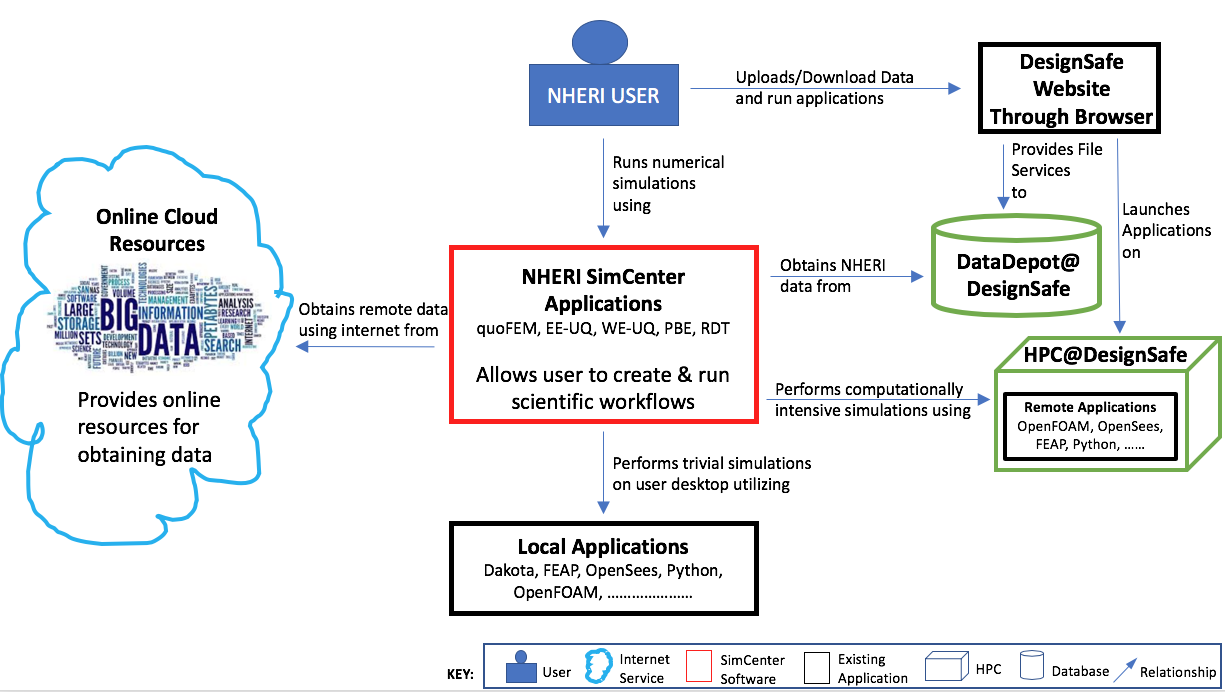
\includegraphics[width=0.95\textwidth]
    {images/context.png} }
  \caption{System Context Diagram for SimCenter Applications}
  \label{fig:context}
\end{figure}


\section{Level 2:  The Components of a SimCenter Application}

Given how SimCenter applications fit in with the environment, a level 2 diagrams now demonstrates how the SimCenter applications are broken into high level components. The SimCenter applications are, as shown in \Cref{fig:container}, broken into two components: A front end UI and a back end application that runs the workflow. The front end applications are desktop applications written using the cross-platform Qt framework. The back end is an application that processes the input from the front end, which comes in the form of a JSON file, creates a workflow and runs it. The workflow applications, written in Python, C, or C++, utilize existing applications were possible and run on either the local desktop machine or on a HPC utilizing resources made available to NHE community through DeisignSafe. 


\begin{figure}[!htbp]
  \centering {
    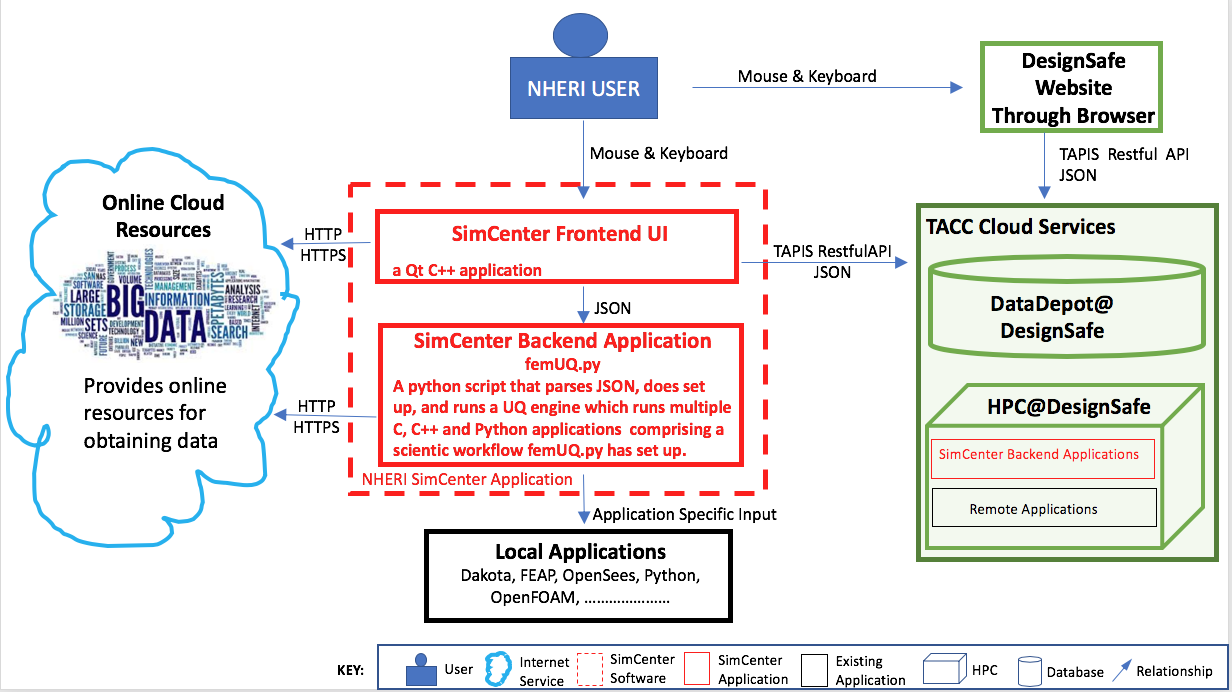
\includegraphics[width=0.95\textwidth]
    {images/container.png} }
  \caption{System Container Diagram for SimCenter Applications}
  \label{fig:container}
\end{figure}

 

\section{Level 3: Container Diagrams for the Front and Back End Components}

Two level 3 diagrams are now presented which break up the two containers into the major building blocks or components in C4 terminology. In \Cref{fig:componentFront} the component diagram for the front end UI is presented. It outlines the interaction between the user and the individual graphical elements (widgets) of the UI. Given the analogy of a jigsaw puzzle, the user selects which piece of the jigsaw puzzle they are working on in the component selection widget. The widget for the jigsaw piece will then be displayed on the desktop. The user for each jigsaw piece then selects which application to run for that piece, and for the chosen application, they provide the inputs. When the inputs are all provided, the user can select to run the simulations locally or remotely. For jobs that run remotely, the user can download and review previously run simulations. As seen the widgets may subsequentially interact with web services through HTTPS requests, or with DesignSafe utilizing TAPIS Restful API through the RemoteService container.



\begin{figure}[!htbp]
  \centering {
    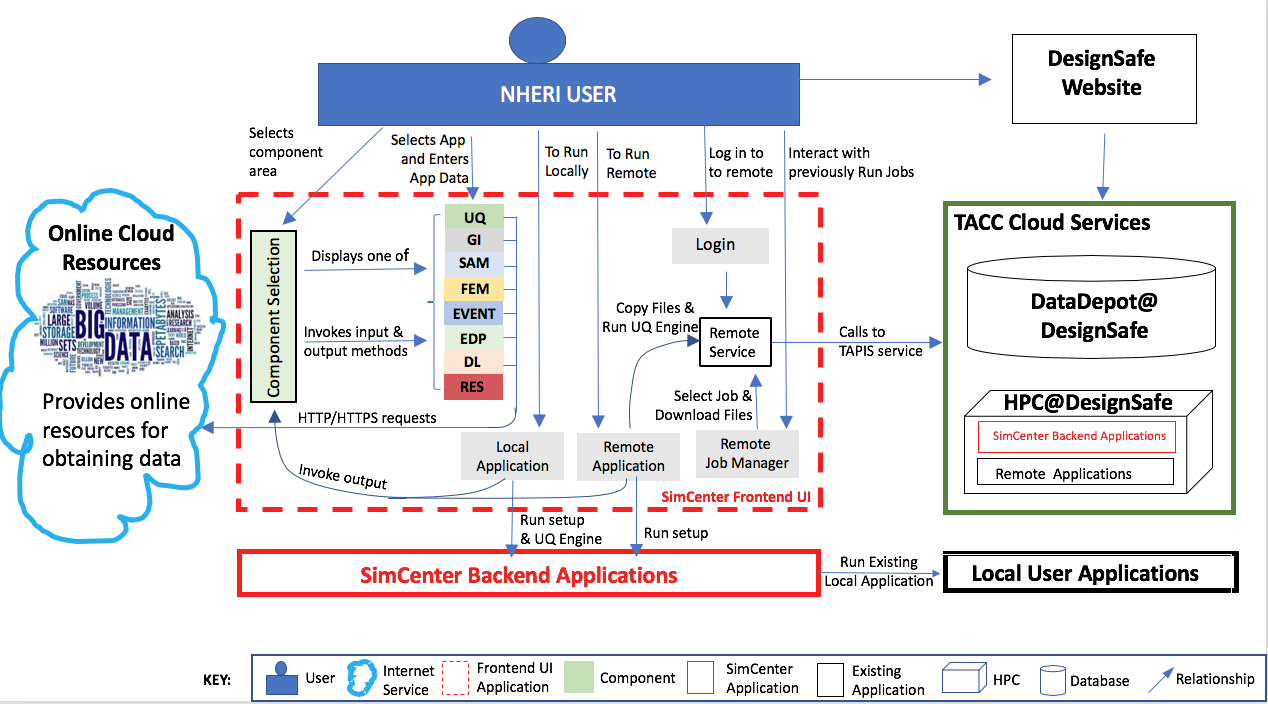
\includegraphics[width=0.95\textwidth]
    {images/componentFront.png} }
  \caption{Component Diagram for Front End UI}
  \label{fig:componentFront}
\end{figure}

 

The component diagram for the backend application shown in \Cref{fig:componentBack}, shows that the backend is made up of a number of component, all applications. The application “femUQ.py” is the application that parses the input from the front end, sets up the workflow and launches the UQ engine. Which UQ Engine and which applications to run in the workflow, is determined from the data passed from the UI and information contained in a WorkflowApplication.json file. A file is used to allow the researchers to modify the applications that may be run in the workflow w/o the need to recompile the application. Control is then passed to a UQ Engine, which repeatedly runs the workflow to generate the results. In running the workflow some of the applications will invoke applications not developed to meet the API. For such applications pre- and post-processors are provided.
The figure shows the backend application running locally or remotely on a HPC@DesignSafe.

 

\begin{figure}[!htbp]
  \centering {
    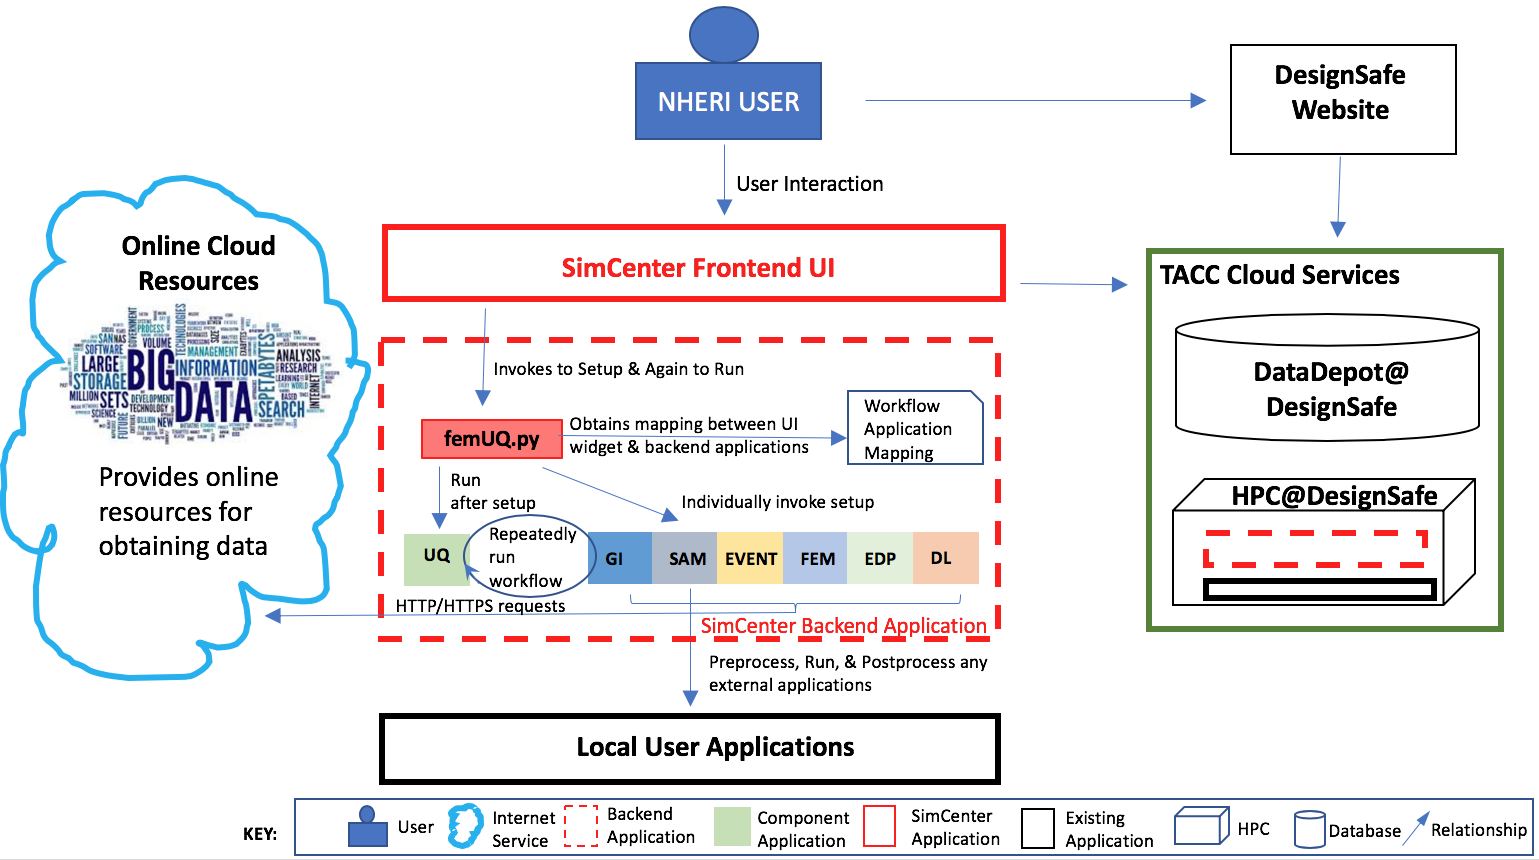
\includegraphics[width=0.95\textwidth]
    {images/componentBack.png} }
  \caption{Component Diagram for Backend Application}
  \label{fig:componentBackEnd}
\end{figure}
 
 
For the UI component of the application currently released, we now present the UML diagrams for each of the major tools that have been released. The function of these tools, as mentioned ad nausiasm, is described in the project execution plan, the work breakdown schedule, the yearly work plan, and the documentation for the application, and is repeated again here.

\section{Level 4 UML Diagrams}

A number of diagrams are presented for the level 4 diagrams. These are mostly UML diagrams showing how the applications are built. The SimCenter releases a number of front-end applications: EE-UQ shown in \Cref{fig:umlEE}, WE-UQ shown in \Cref{fig:umlWE}, and PBE shown in \Cref{fig:umlPBE}. These applications share code with each other and other SimCenter applications. As a consequence, the common code is bundled into a number of shared packages: EarthquakeEvents shown in \Cref{fig:umlEarthquakeEvents}, WindEvents shown in \Cref{fig:umlWindEvents}, and SimCenterCommon shown in \Cref{fig:umlCommon}. A number of packages were chosen over placing all common code inside a single package to simplify development efforts for outside programmers (whom it is envisioned will mostly be adding new event components) and to reduce the overhead of package management and compile time for SimCenter programmers. UML diagrams are  presented for these front-end applications and shared packages. THE UML diagrams that are presented are not exhaustive, in that they do not show all classes used, for it was decided not to for example show the myriad of Line edits, labels, spin boxes, etc. that make up the widgets. What is shown is sufficient to present the SimCenter architecture.

While there are a number of different types of UML diagrams,  those shown in this document will be limited to class diagrams and sequence diagrams. SimCenter applications are object-oriented in nature. An object-oriented program consists of objects interacting with one another,  with each object being of a certain type or class. A class diagram shows the classes, their attributes and methods, and the relationships between the classes. A sequence diagram or event diagram shows the order in which objects interact. To understand the SimCenter framework it is useful to first present the main() function for a SImCenter application, in this case EE-UQ, shown in \Cref{fig:mainCode}. The code presentebd is a stripped down version of the actual code, code for dealing with style sheets, analytics, etc. is not shown as it is not pertinent to understanding of the software architecture.


\begin{verbatim}
int main(int argc, char *argv[]) {

    QApplication app(argc, argv);
 
    //                                                                       
    // create a remote interface                                             
    //                                                                       

    QString tenant("designsafe");
    QString storage("agave://designsafe.storage.default/");
    QString dirName("EE-UQ");
    
    //                                                                       
    // create the main window                                                
    // 
    
    WorkflowAppWidget *theInputApp = new WorkflowAppEE_UQ(theRemoteService);
    MainWindowWorkflowApp window(QString("EE-UQ: Response of Building to Earthquake"), theInputApp, theRemoteService);
    
    windows.setVersion("Version 1.0.0");


    //                                                                       
    // move remote interface to a thread                                     
    //                                                                       

    QThread *thread = new QThread();
    theRemoteService->moveToThread(thread); 
    thread->start();

    //                                                                       
    // show the main window, set styles & start the event loop               
    //                                                                       

    window.show(); 
    int res = app.exec();

    //                                                                       
    // on done with event loop, logout & stop the thread                     
    //                                                                       

    theRemoteService->logout();
    thread->quit();
    
     return res;
}
 \end{verbatim}
 \begin{figure}
  \caption{main function for EE-UQ}
  \label{fig:mainCode}
 \end{figure}

As was mentioned the Front end UI applications are built using Qt. In a Qt application the programmer creates a QApplication object, in \Cref{fig:mainCode} the object named \begin{verbatim}app\end{verbatim} and a QMainWindow, in the example named \begin{verbatim}window\end{verbatim}. As will be shown in \Cref{fig:umlCommon} MainWindowWorkflowApp is a type of QMainWindow that is used in all SimCenter research applications as it deals with all the application menu items, e.g. File open and close, Help cite, etc The QMainWindowWorkflowApp is a SImCenter class that contains a single QWidget of type WorkflowAppWidget. The WorkflowAppWidget object is passed a RemoteService, the remote cloud service that the application will interact with. This RemoteService is placed in it's own QThread object, so that the UI can respond to user requests while communication with cloud service is underway. Once the window object is shown, control is passed to the QApplication  until the user is done.
For EE-UQ the type of WorkflowAppWidget is of type WorkflowAppEE-UQ, which is shown in \Cref{fig:umlEE}. Other applications have their own subclasses of WorkflowAappWidget.

\subsection{EE-UQ}

EE-UQ is an application to determine the response of a building subjected to an earthquake event. As shown in \Cref{fig:umlEE} it comprises a component selection which presents the user with a a number of components, jigsaw pieces, which include: earthquake event (EarthquakeEventSelection), UQ engine (UQ Selection), demand parameters of inters (EDP Selection), building information model (BIM Selection),  strutctural analysis model generator (SAM Selection), finite element application (FEM Selection), and RandomVariableContainer.  RandomVariableContainer is a widget allowing user to specify distrubutions associated with the random variables created by user. As will be seen in \Cref{fig:umlEarthquakeEvents} and \Cref{fig:umlCommon} each component offers the user a number of applications to choose from for that component. Other classes corresponding to widgets presented in the Front end UI include: UQ Result for displaying the results, Local and Remote Services for running the job locally or remotely, Remote job Manager for monitoring job status and retrieving old jobs, and Login for obtaining credentials from DesignSafe to access and run jobs on the HPC resources. All communication between the applications and DesignSafe-ci is through the Application Service. This is done to allow the applications to switch to other cloud service providers, possibly allowing applications to run at DesignSafe, on Amazon EC-2, IBM's Azure or elsewhere.

 \begin{figure}[!htbp]
  \centering {
    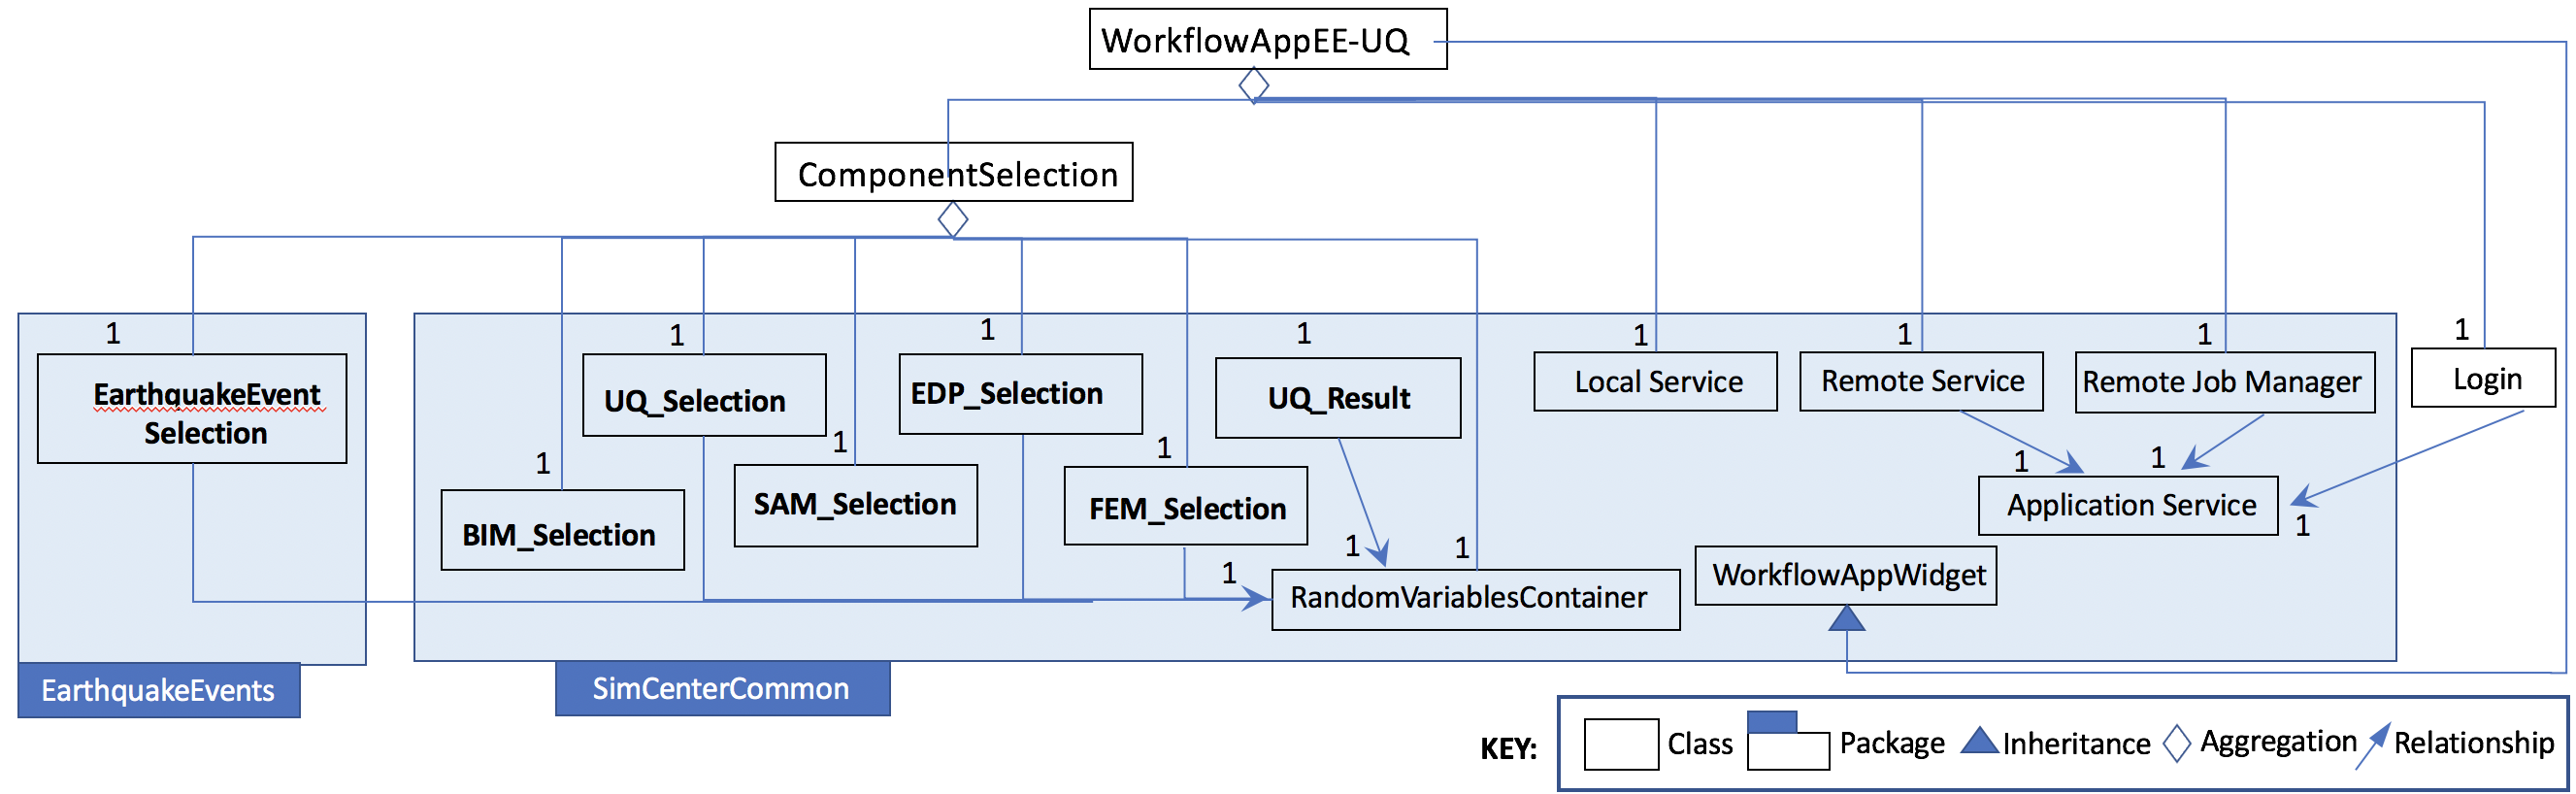
\includegraphics[width=0.95\textwidth]
    {images/umlEE.png} }
  \caption{UML Diagram for EU-UQ}
  \label{fig:umlEE}
\end{figure}


\subsection{WE-UQ}
Similar in  construction to EE-UQ is WE-UQ, as shown in figure \Cref{fig:umlWE}.  In fact the only difference is that Wind Event Selection is present in the component selection, instead of Earthquake Events. The wind event applications, as will be shown in \Cref{fig:windEvents} include stochastic wind models, wind loading from online services such as Vortex-Winds, applications which take online wind tunnel experimental datasets such as those from Tokyo Polytechnic.


 \begin{figure}[!htbp]
  \centering {
    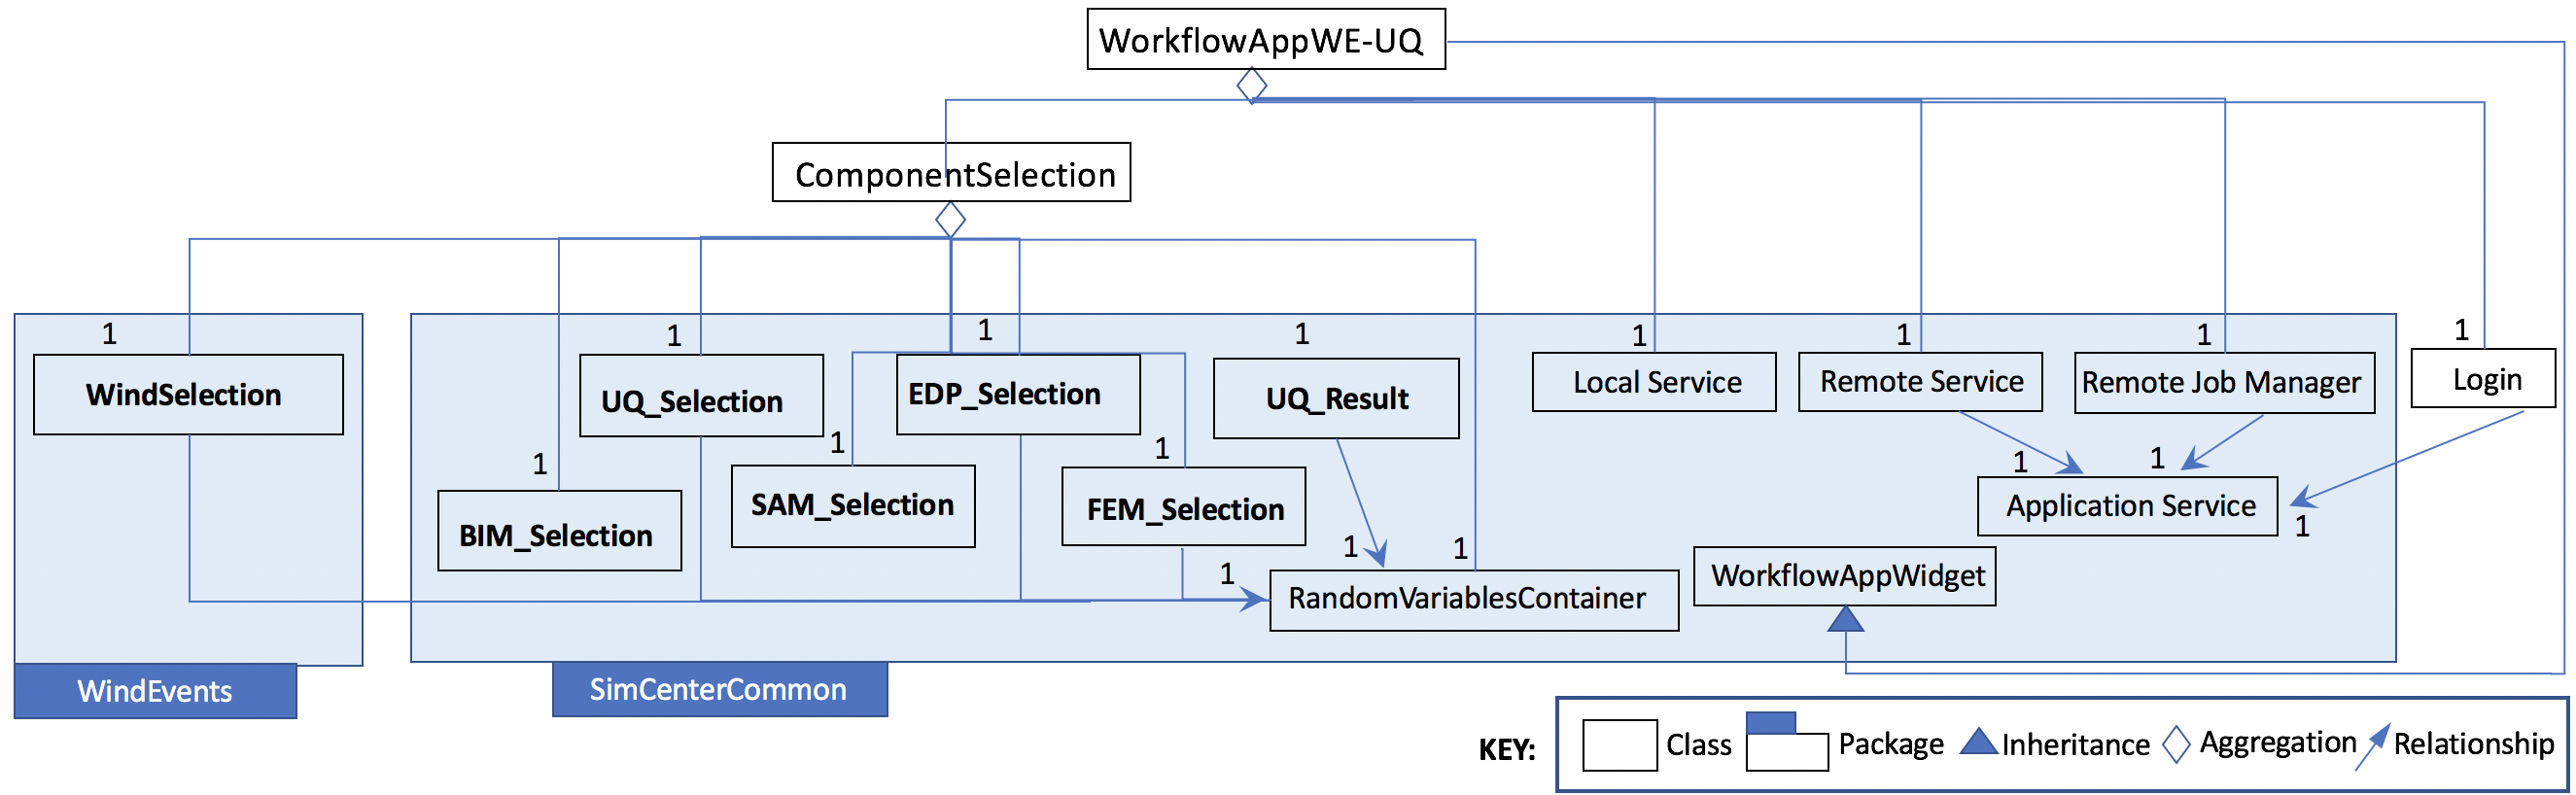
\includegraphics[width=0.95\textwidth]
    {images/umlWE.png} }
  \caption{UML Diagram for WU-UQ}
  \label{fig:umlWE}
\end{figure}

 

\subsection{PBE}

 PBE is a tool for performance based engineering. Given a building and an event it will calculate downtime and loss estimates. As can be sen in \Cref{fig:umlPBE},  it adds a LossModelSelection to the component Selections available in EE-UQ. In future it, or another application, will add similar for WE-UQ.
The Loss Model applications currently available for selection include a a P58 Loss Model and a HAZUS Loss Model. Depending on selection, deifferent widgets are presented for the user to input the different input arguments needed for the different loss model calculations. Presently the calculations for both loss models are perforrmed by the same python script, CalculateDL.py, in the collection of backend applications.
 
 \begin{figure}[!htbp]
  \centering {
    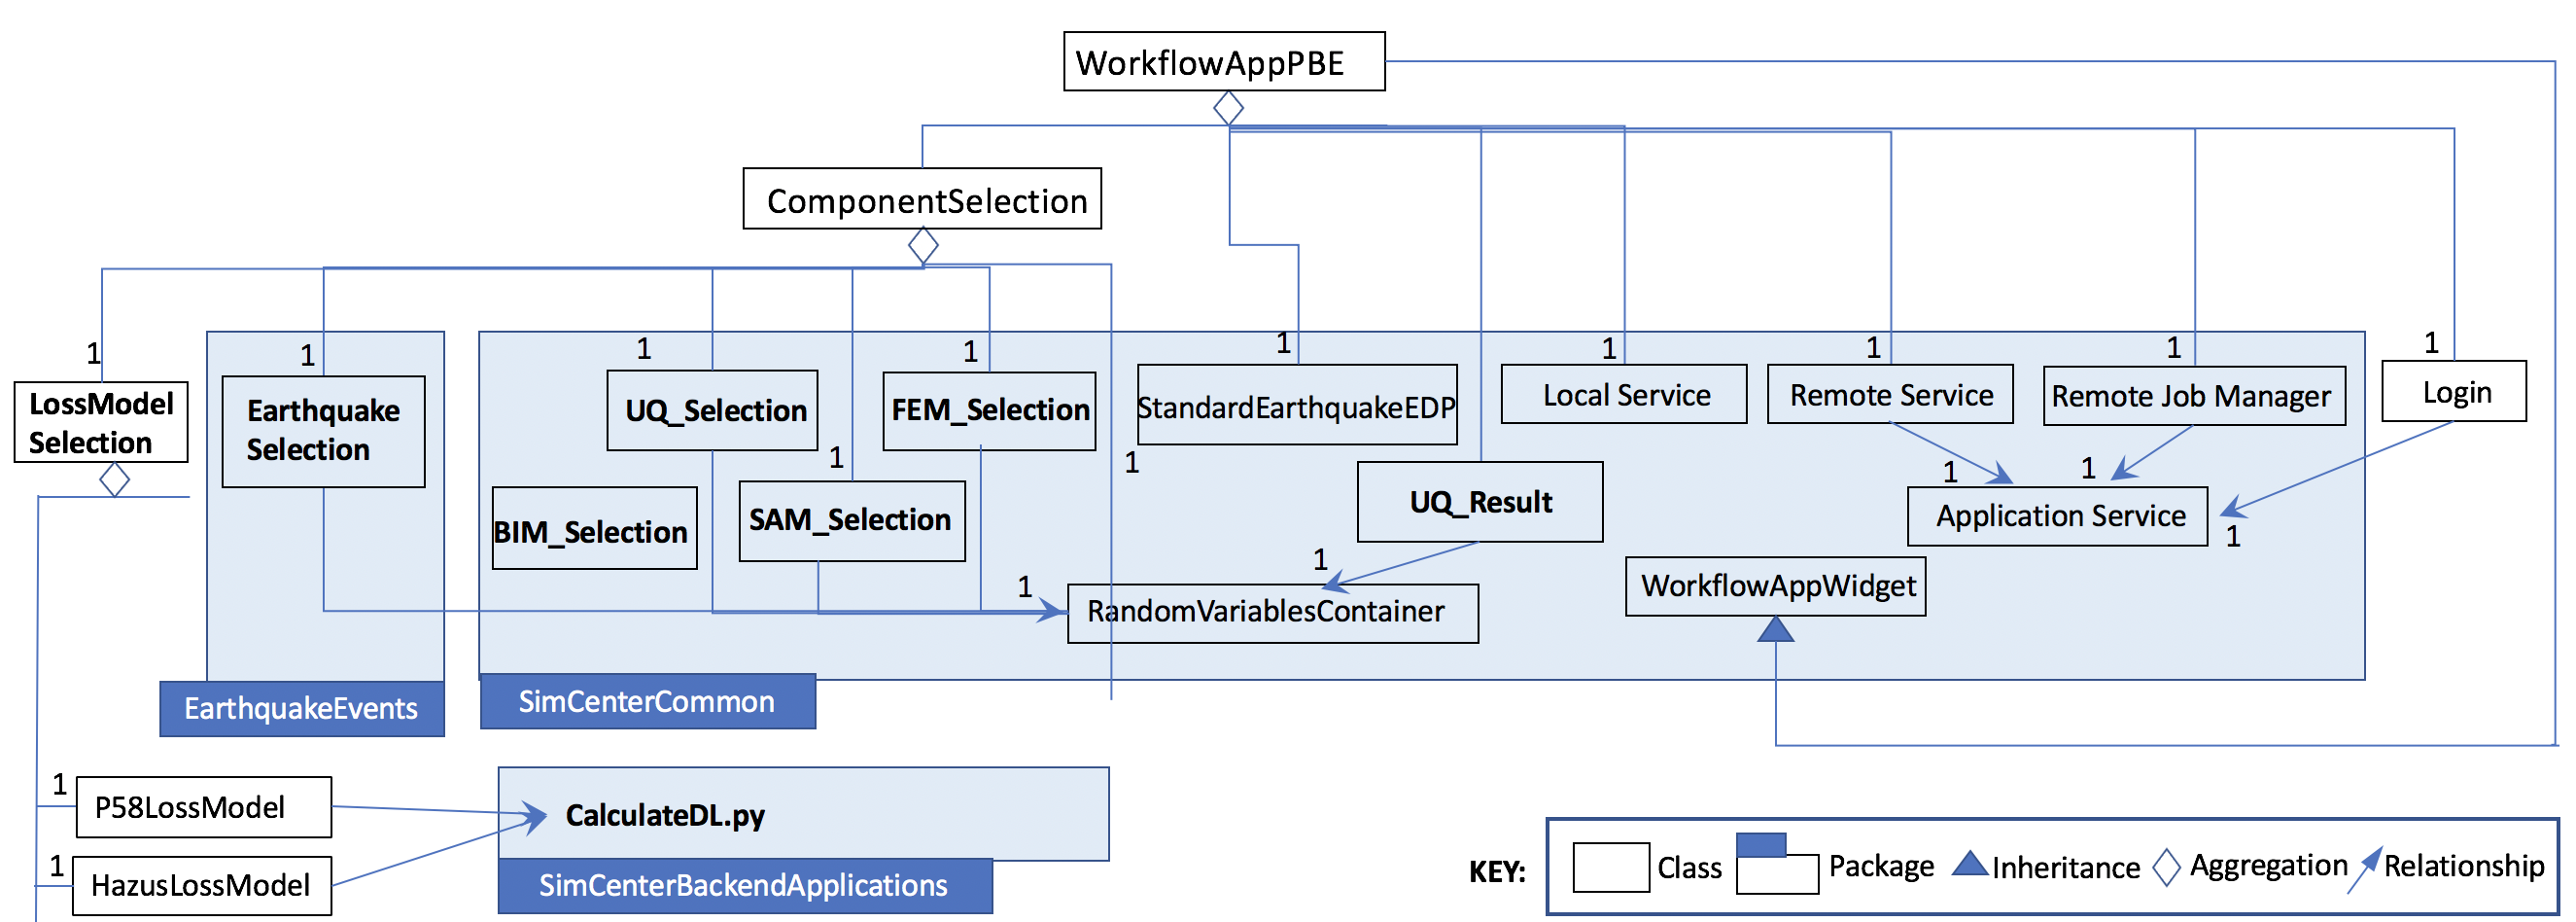
\includegraphics[width=0.95\textwidth]
    {images/umlPBE.png} }
  \caption{UML Diagram for PBE}
  \label{fig:umlPBE}
\end{figure}
 

\subsection{EarthquakeEvents}
 The Earthquake Events package, as shown in \Cref{fig:umlEarthquakeEvents}, contains an Earthquake Event selector with a number of Earthquake Event selections available. The selections include options that interface with the NGA west server directly and options that will collect inputs for stochastic input models of Vlachos et Al or Dabahi and DerKiuerghian, peer NGA records, site response and our own SimCenterEvent format. Each of these widgets corresponds to one application in the backend, e.g. RockOutcrop corresponds to SiteReponse, and it is this application that will run when the workflow runs.

 
 \begin{figure}[!htbp]
  \centering {
    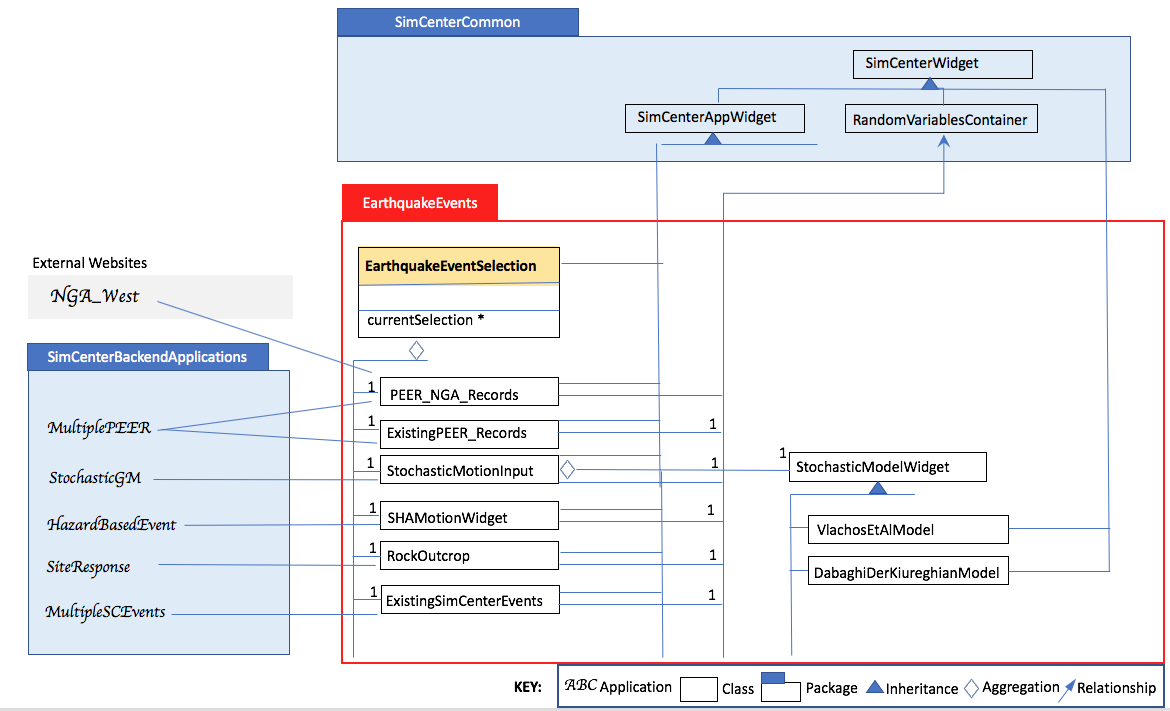
\includegraphics[width=0.95\textwidth]
    {images/umlEarthquakeEvents.png} }
  \caption{UML Diagram for Earthquake Events}
  \label{fig:umlEarthquakeEvents}
\end{figure}
 
 

\subsection{WindEvents}
Similar to the Earthquake Events package, the wind events package shown in \Cref{fig:umlWindEvents}, contains a WInd Event Selector with a number of Wnd Event selections available. The selections include options for stochastically generated wind events, events that obtain wind loading from the vortex-winds server, options to obtain forces from eind tunnel events, either from the Tokyo Ploytechnic University database, or a user supplied file.

 
  \begin{figure}[!htbp]
  \centering {
    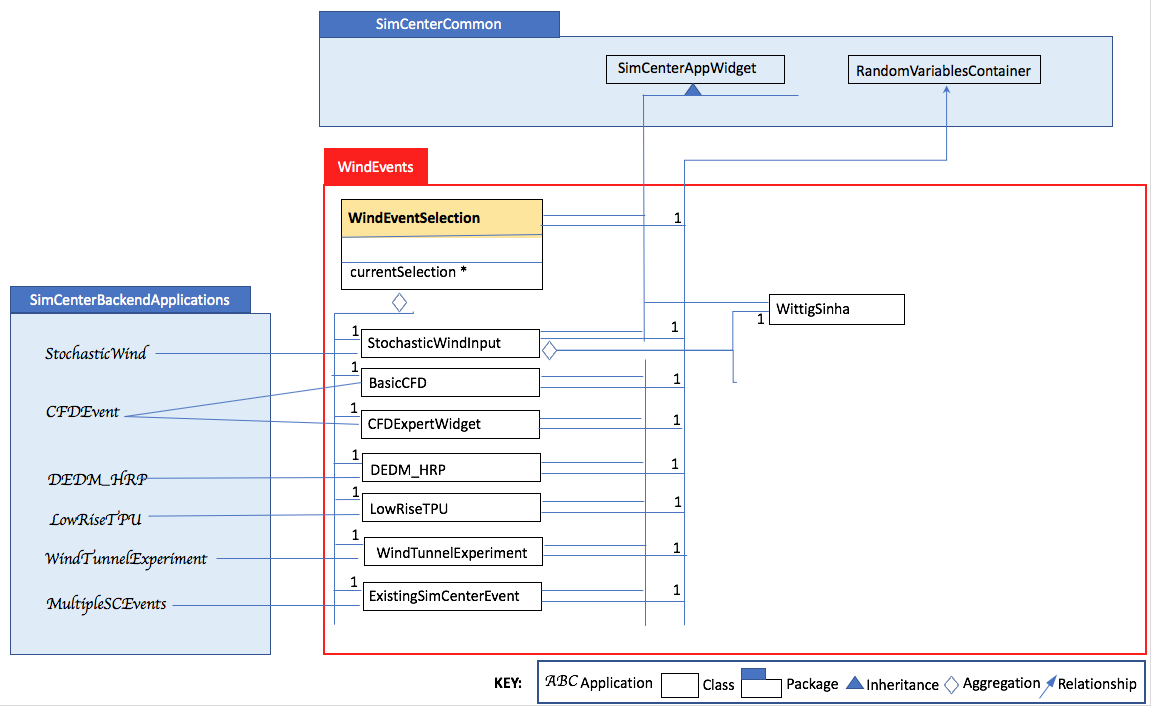
\includegraphics[width=0.95\textwidth]
    {images/umlWindEvents.png} }
  \caption{UML Diagram for Wind Events}
  \label{fig:umlWindEvents}
\end{figure}
 

\subsection{SimCenterCommon}
SimCenter common shown in \Cref{fig:umlCommon} contains a number of component selctions, BIM selection, EDP Selection, SAM Selection, FEM Selection and UQ Engine Selection. Each contains a number of options. The components and their options are all subclasses of the SImCenterAppWidget class, The SImCenterAppWidget has methods to output and input from a JSON object. SimCenterCommon also contains the RandomVariablesContainer class, each object being a container for a number of RandomVariables. Each RansomVariable having a name and a RandomVariable Distribution associated with it. Types of RandomVariableDistributions include for exmaple Normal, Lognormal, Uniform, Beta, and Gumbel.

 

\begin{figure}[!htbp]
  \centering {
    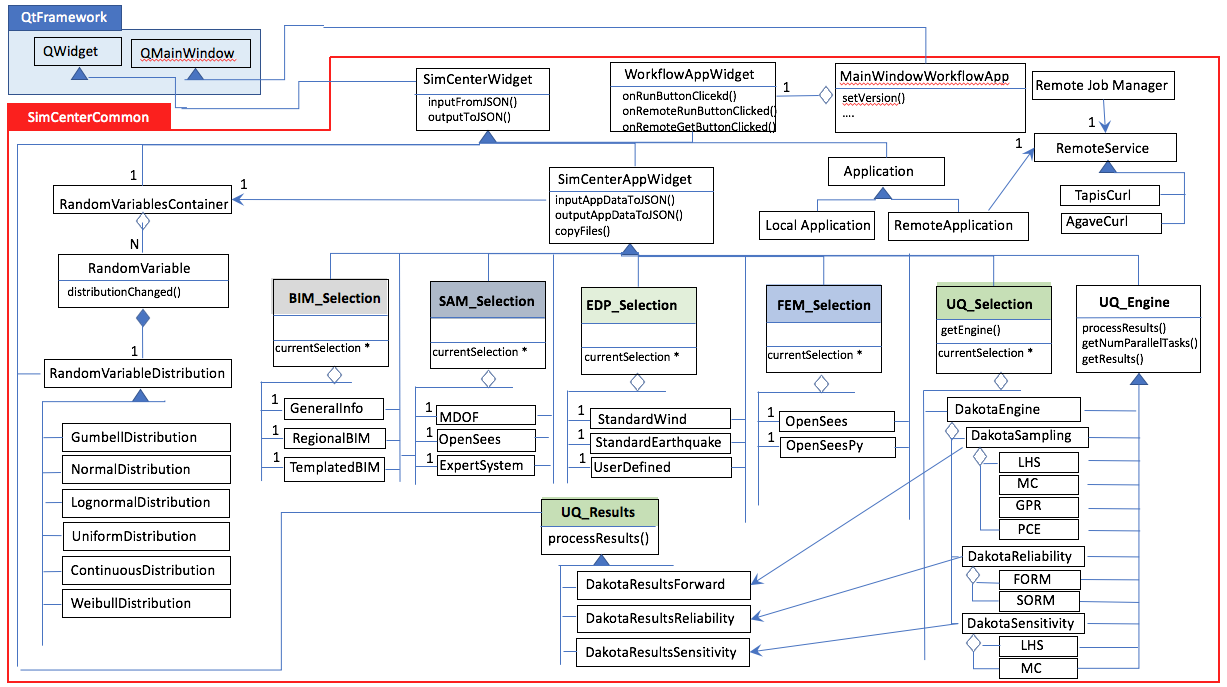
\includegraphics[width=0.95\textwidth]
    {images/umlCommon.png} }
  \caption{UML Diagram for SimCenter Common}
  \label{fig:umlCommon}
\end{figure}
 


\subsection{SimCenter Backend Applications}

The BackendApplications are currently all in a single package. These are the applications that perform the numerical computations when the workflow runs. Some of these applications rely on external applications, websites, and external packages.  The external applications, web services, and libraries are as shown in \Cref{fig:appDiagramBackend}


\begin{figure}[!htbp]
  \centering {
    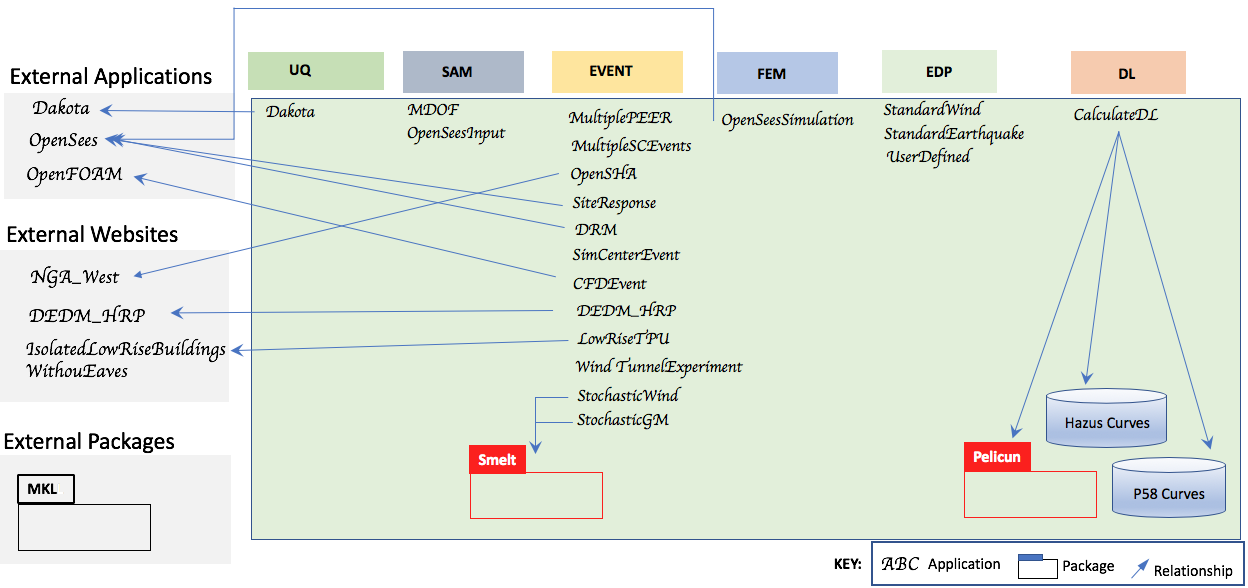
\includegraphics[width=0.95\textwidth]
    {images/appDiagramBackend.png} }
  \caption{Applications for Backend Applications}
  \label{fig:appDiagramBackend}
\end{figure}
 



\chapter{Data Gathering Applications}
\label{chap:about}
Additional tools are being developed for the regional simulations. These applications are needed to create the knowledge bases used for the built environment in the regional simulations. While not complicated in design, these applications are useful for NHERI researchers to gather additional information. This chapter contains up to a level 3 description of the software.

\section{Level 1: Context for Data Gathering Backend Applications}

A level 1 description showing the context of the software provided for data gathering is shown in \Cref{fig:contextData}. It shows that the software uses information available on the WWW to build the datasets.

 \begin{figure}[!htbp]
  \centering {
    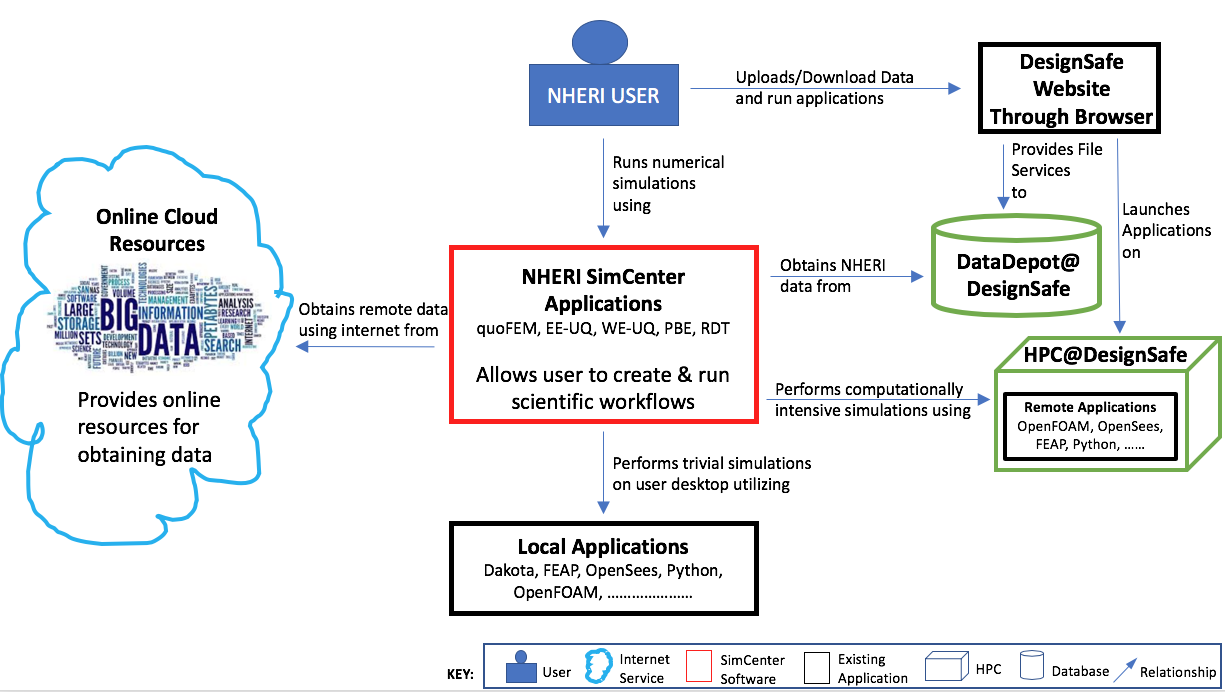
\includegraphics[width=0.95\textwidth]
    {images/context.png} }
  \caption{System Context Diagram for Data Gathering Applications}
  \label{fig:contextData}
\end{figure}

\section{Level 2: Container Diagram for Data Gathering Applications}
A level 2 container diagram shows that this software is again broken into 2; initial software to ascertain parcel level building information and then software to collect additional data.

\begin{figure}[!htbp]
  \centering {
    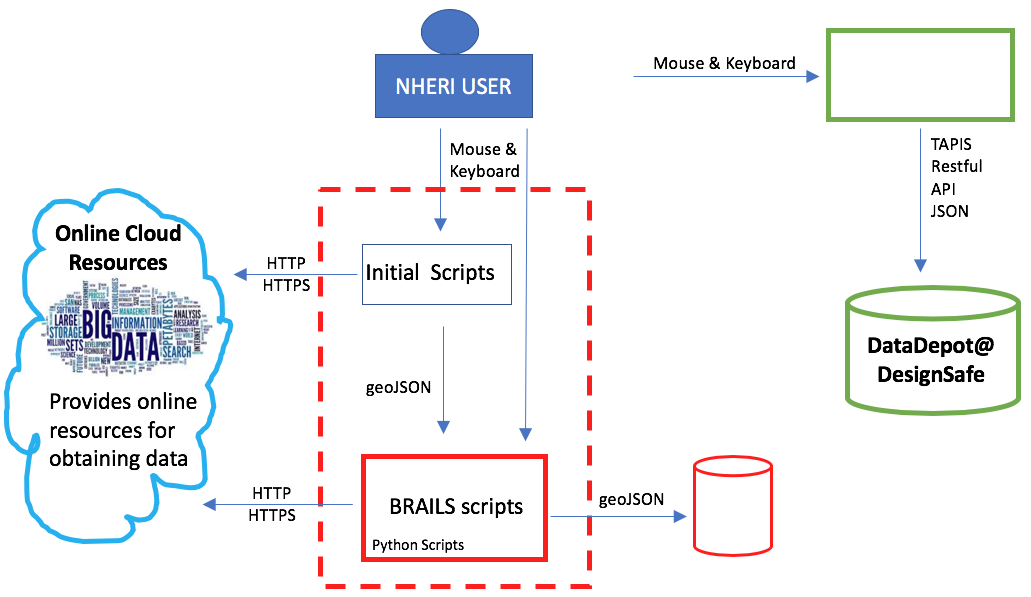
\includegraphics[width=0.95\textwidth]
    {images/containerData.png} }
  \caption{System Container Diagram for Data Gathering Applications}
  \label{fig:containerData}
\end{figure}

 
\section{Level 3: Component Diagram for BRAILS container}

A number of applications are provided, some of which utilize Selenium to scrape assessors’ databases for information at the parcel level on building data. Some applications utilize Machine learning to ascertain building properties, e.g. roof shapes and first floor levels. These applications, and trained neural networks are included in the BRAILS framework. The applications cannot ascertain all the information for the regional datasets. Where information is missing SURF.ET-AI.py is used. SURF.ET-AI.py is part of SURF package. SURF is used to fill in the missing data.
 
\begin{figure}[!htbp]
  \centering {
    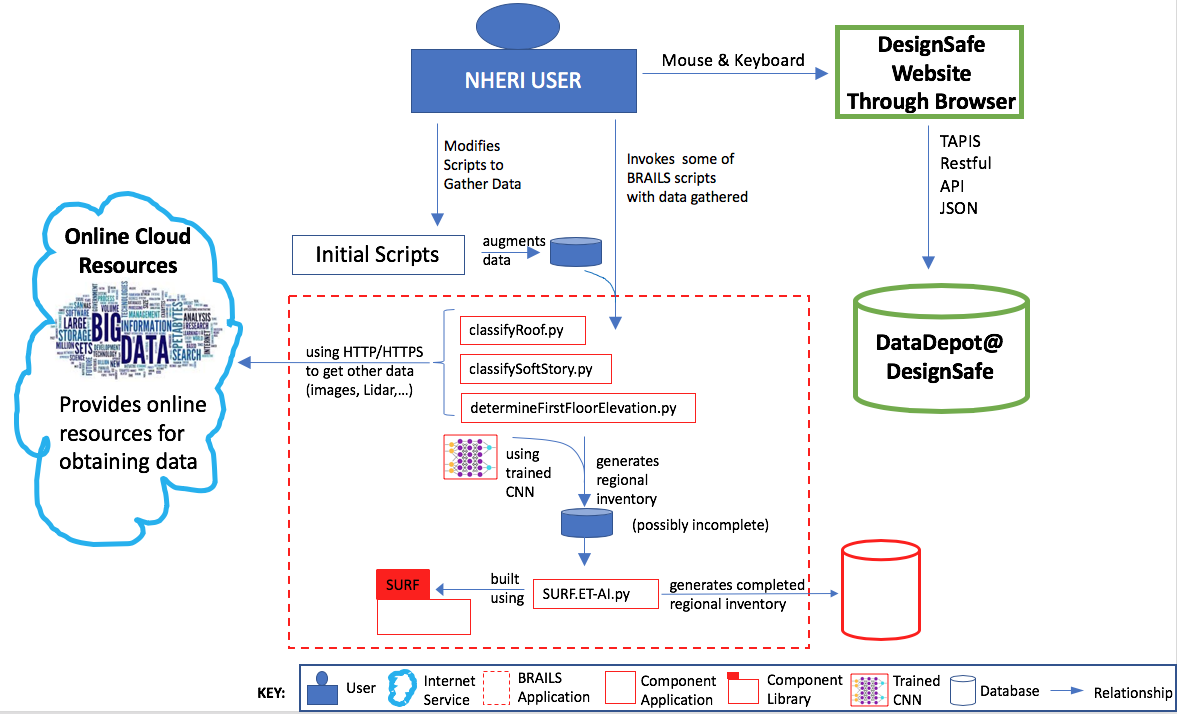
\includegraphics[width=0.95\textwidth]
    {images/componentBRAILS.png} }
  \caption{Component Diagram for BRAILS}
  \label{fig:componentBRAILS}
\end{figure}


\chapter{Software Versioning}
\label{chap:versioining}
\input{versioning.tex}

\pagestyle{plain}
{
  \renewcommand{\thispagestyle}[1]{}	
  \printbibliography           
}

\end{document}
